% 這個版本的 CVPR 模板由 Ming-Ming Cheng 提供。
% 如果您發現錯誤,請留下問題:
% https://github.com/MCG-NKU/CVPR_Template。

%\documentclass[review]{cvpr}
\documentclass[final]{cvpr}
\usepackage[UTF8]{ctex}
\usepackage{enumitem}
\usepackage{times}
\usepackage{epsfig}
\usepackage{graphicx}
\usepackage{amsmath}
\usepackage{amssymb}
\usepackage{makecell}
\usepackage{booktabs}
\usepackage[table,xcdraw]{xcolor}
\usepackage{multirow}
\usepackage{bbm}

% 在這裡包含其他套件,在 hyperref 之前。

% 如果您註釋掉 hyperref 然後取消註釋它,您應該刪除
% egpaper.aux 然後重新運行 latex。 (或者只需在第一次 latex 運行時按 'q',讓它完成,您應該就可以了)。
\usepackage[pagebackref=true,breaklinks=true,colorlinks,bookmarks=false]{hyperref}

\def\cvprPaperID{4107} % *** 在此處輸入 CVPR 論文 ID
\def\confYear{CVPR 2021}
%\setcounter{page}{4321} % 僅適用於最終版本

\begin{document}

\title{鐵路不是火車:顯著性作為弱監督語義分割的偽像素監督}

\author{Seungho Lee\thanks{ 表示相同貢獻。}\\
延世大學\\
{\tt\small seungholee@yonsei.ac.kr}
% 對於所有作者都在同一機構的論文,
% 省略以下行,直到關閉“}”。
% 可以使用“\and”添加其他作者和地址,
% 就像第二位作者一樣。
% 為了節省空間,請使用電子郵件地址或主頁,而不是兩者
\and
Minhyun Lee\footnotemark[1]\\
延世大學\\
{\tt\small lmh315@yonsei.ac.kr}
\and 
Jongwuk Lee\\
成均館大學\\
{\tt\small jongwuklee@skku.edu}
\and 
Hyunjung Shim\thanks{Hyunjung Shim 是通訊作者。}\\
延世大學\\
{\tt\small kateshim@yonsei.ac.kr}
}

\maketitle
\thispagestyle{empty}
\pagestyle{empty}

%%%%%%%%% 摘要

\begin{abstract}
現有使用圖像級弱監督的弱監督語義分割(WSSS)研究存在幾個限制:稀疏的物體覆蓋、不準確的物體邊界以及來自非目標物體的共現像素。為了克服這些挑戰,我們提出了一個新穎的框架,即顯式偽像素監督(EPS),通過結合兩種弱監督從像素級反饋中學習;圖像級標籤通過定位圖提供物體身份,來自現成顯著性檢測模型的顯著性圖提供豐富的邊界。我們設計了一種聯合訓練策略,以充分利用兩種信息之間的互補關係。我們的方法可以獲得準確的物體邊界並丟棄共現像素,從而顯著提高偽掩碼的質量。實驗結果表明,所提出的方法通過解決 WSSS 的關鍵挑戰顯著優於現有方法,並在 PASCAL VOC 2012 和 MS COCO 2014 數據集上實現了新的最先進性能。代碼可在 \href{https://github.com/halbielee/EPS}{https://github.com/halbielee/EPS} 獲得。
\end{abstract}


\section{介紹}

弱監督語義分割(WSSS)利用弱監督(例如,圖像級標籤~\cite{pathak2015constrained, pinheiro2015image}、塗鴉~\cite{lin2016scribblesup} 或邊界框~\cite{khoreva2017simple})並旨在實現與完全監督模型相媲美的性能,這需要像素級標籤。大多數現有研究採用圖像級標籤作為分割模型的弱監督。WSSS 的整體流程由兩個階段組成。首先,使用圖像分類器為目標物體生成偽掩碼。然後,使用偽掩碼作為監督訓練分割模型。生成偽掩碼的流行技術是類激活映射(CAM)~\cite{zhou2016learning},它提供與其圖像級標籤對應的物體定位圖。由於完全(即像素級註釋)和弱(即圖像級標籤)監督語義分割之間的監督差距,WSSS 存在以下關鍵挑戰:1)定位圖僅捕獲目標物體的一小部分~\cite{zhou2016learning},2)它遭受物體邊界不匹配的困擾~\cite{kim2017two},以及 3)它幾乎無法將共現像素與目標物體分開(例如,鐵路與火車)~\cite{kolesnikov2016seed}。

\begin{figure}[t]
\centering
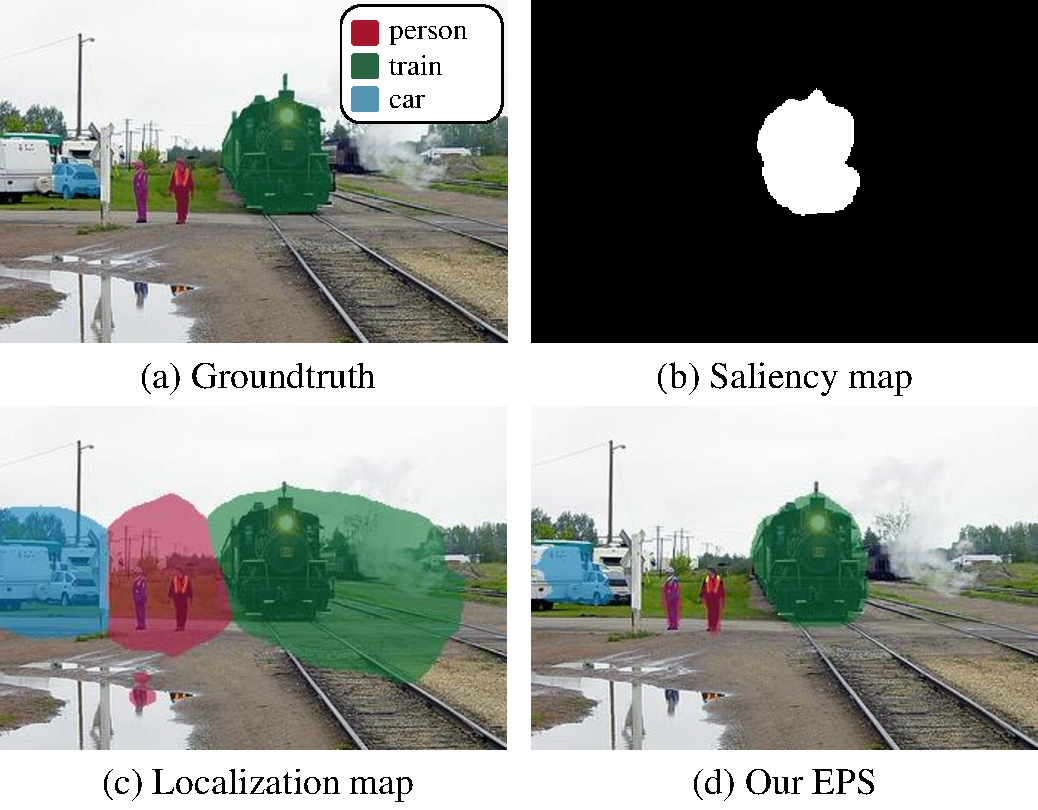
\includegraphics[width=8 cm]{figures/fig_concept.pdf}
\caption{Motivating example of utilizing both the saliency map and the localization map for WSSS. (a) Groundtruth, (b) saliency map via PFAN~\cite{zhao2019pyramid}, (c) localization map via CAM~\cite{zhou2016learning} and (d) our EPS utilizing both the saliency map and the localization map for training a classifier. Note that the saliency map cannot capture \emph{person} and \emph{car} while our result can correctly restore them, and the localization map overly captures two objects.} \vspace{-2mm}
\label{fig:concept}
\end{figure}

為了解決這些問題,現有的研究可以分為三個支柱。第一種方法是通過擦除像素~\cite{choe2020attention,kim2017two, li2018tell}、集成得分圖~\cite{jiang2019integral, lee2019ficklenet}或使用自監督信號~\cite{wang2020self}來擴展物體覆蓋範圍以捕捉物體的全部範圍。然而,由於缺乏引導物體形狀的線索,它們無法確定目標物體的準確邊界。第二種方法專注於改善偽掩膜的物體邊界~\cite{fan2020learning,chen2020boundary}。由於它們有效地學習了物體邊界,因此自然地將偽掩膜擴展到邊界。然而,它們仍然無法區分非目標物體與目標物體的重合像素。這是因為前景和背景之間的強相關性(即,共現)幾乎無法從歸納偏差中區分出來(即,觀察到目標物體及其重合像素的頻率),如~\cite{choe2020evaluating}所示。最後,第三種方法旨在使用額外的真實掩膜~\cite{BMVC2016_92}或顯著性圖~\cite{oh2017exploiting, yao2020saliency}來緩解共現問題。然而,\cite{BMVC2016_92,li2018tell}需要強像素級註釋,這與弱監督學習範式相去甚遠。\cite{oh2017exploiting}對顯著性圖的錯誤非常敏感。此外,\cite{yao2020saliency}無法覆蓋物體的全部範圍,並且存在邊界不匹配的問題。

在本文中,我們的目標是通過充分利用定位圖(即,使用圖像級標籤訓練的圖像分類器的CAM)和顯著性圖(即,現成的顯著性檢測模型的輸出~\cite{hou2017deeply,nguyen2019deepusps,zhao2019pyramid})來克服WSSS的三個挑戰。我們專注於定位圖和顯著性圖之間的互補關係。如圖~\ref{fig:concept}所示,定位圖可以區分不同的物體,但無法有效地分離它們的邊界。相反,雖然顯著性圖提供了豐富的邊界信息,但它並未揭示物體的身份。在這個意義上,我們認為我們的方法使用兩個互補的信息可以解決WSSS的性能瓶頸。

為此,我們提出了一種新的WSSS框架,稱為\emph{顯式偽像素監督(EPS)}。為了充分利用顯著性圖(即,前景和背景),我們設計了一個分類器來預測$C+1$類,包含$C$個目標類和背景類。我們利用$C$個定位圖和背景定位圖來估計顯著性圖。然後,顯著性損失被定義為顯著性圖和我們估計的顯著性圖之間的像素差異。通過引入顯著性損失,模型可以通過所有類的偽像素反饋進行監督。我們還使用多標籤分類損失來預測圖像級標籤。因此,我們訓練分類器以優化顯著性損失和多標籤分類損失,協同優化背景和前景像素的預測——我們發現我們的策略可以改善顯著性圖(第~\ref{section3.3}節和圖~\ref{fig:sal})和偽掩膜(第~\ref{section:5.1}節和圖~\ref{fig:ablation})。

我們強調,由於顯著性損失通過偽像素反饋懲罰邊界不匹配,它可以強制我們的方法學習物體的準確邊界。作為副產品,我們還可以通過將地圖擴展到邊界來捕捉整個物體。由於顯著性損失有助於將前景(例如,火車)與背景分開,我們的方法可以將共現像素(例如,鐵路)分配到背景類。實驗結果表明,我們的EPS在PASCAL VOC 2012和MS COCO 2014數據集上取得了顯著的分割性能,創造了新的最先進的準確性記錄。

\section{相關工作}

\noindent\textbf{弱監督語義分割。}
WSSS 的一般流程是從分類網絡生成偽掩碼,並使用偽掩碼作為監督來訓練分割網絡。由於圖像級標籤中邊界信息的稀缺,許多現有方法遭受於不準確的偽掩碼。為了解決這個問題,交叉圖像親和性~\cite{fan2020cian}、知識圖譜~\cite{liu2020leveraging} 和對比優化~\cite{sun2020mining, zhang2020splitting} 被用來提高偽掩碼的質量。\cite{chang2020weakly} 提出了一個自監督任務來發現子類別,以強化分類器來改進 CAM。\cite{ahn2019weakly, ahn2018learning} 通過計算像素之間的親和性來隱式利用邊界信息。\cite{zhang2020reliability} 專注於生成可靠的像素級註釋,並設計了一個端到端的網絡來生成分割圖。\cite{huang2018weakly, kolesnikov2016seed} 通過利用邊界損失來訓練分割網絡。最近,\cite{araslanov2020single} 使用了一個基於單一分割的模型,並採用自監督訓練方案。\cite{fan2020employing} 通過利用多個不完整的偽掩碼來專注於分割網絡的魯棒性。

\begin{figure*}[t]
\centering
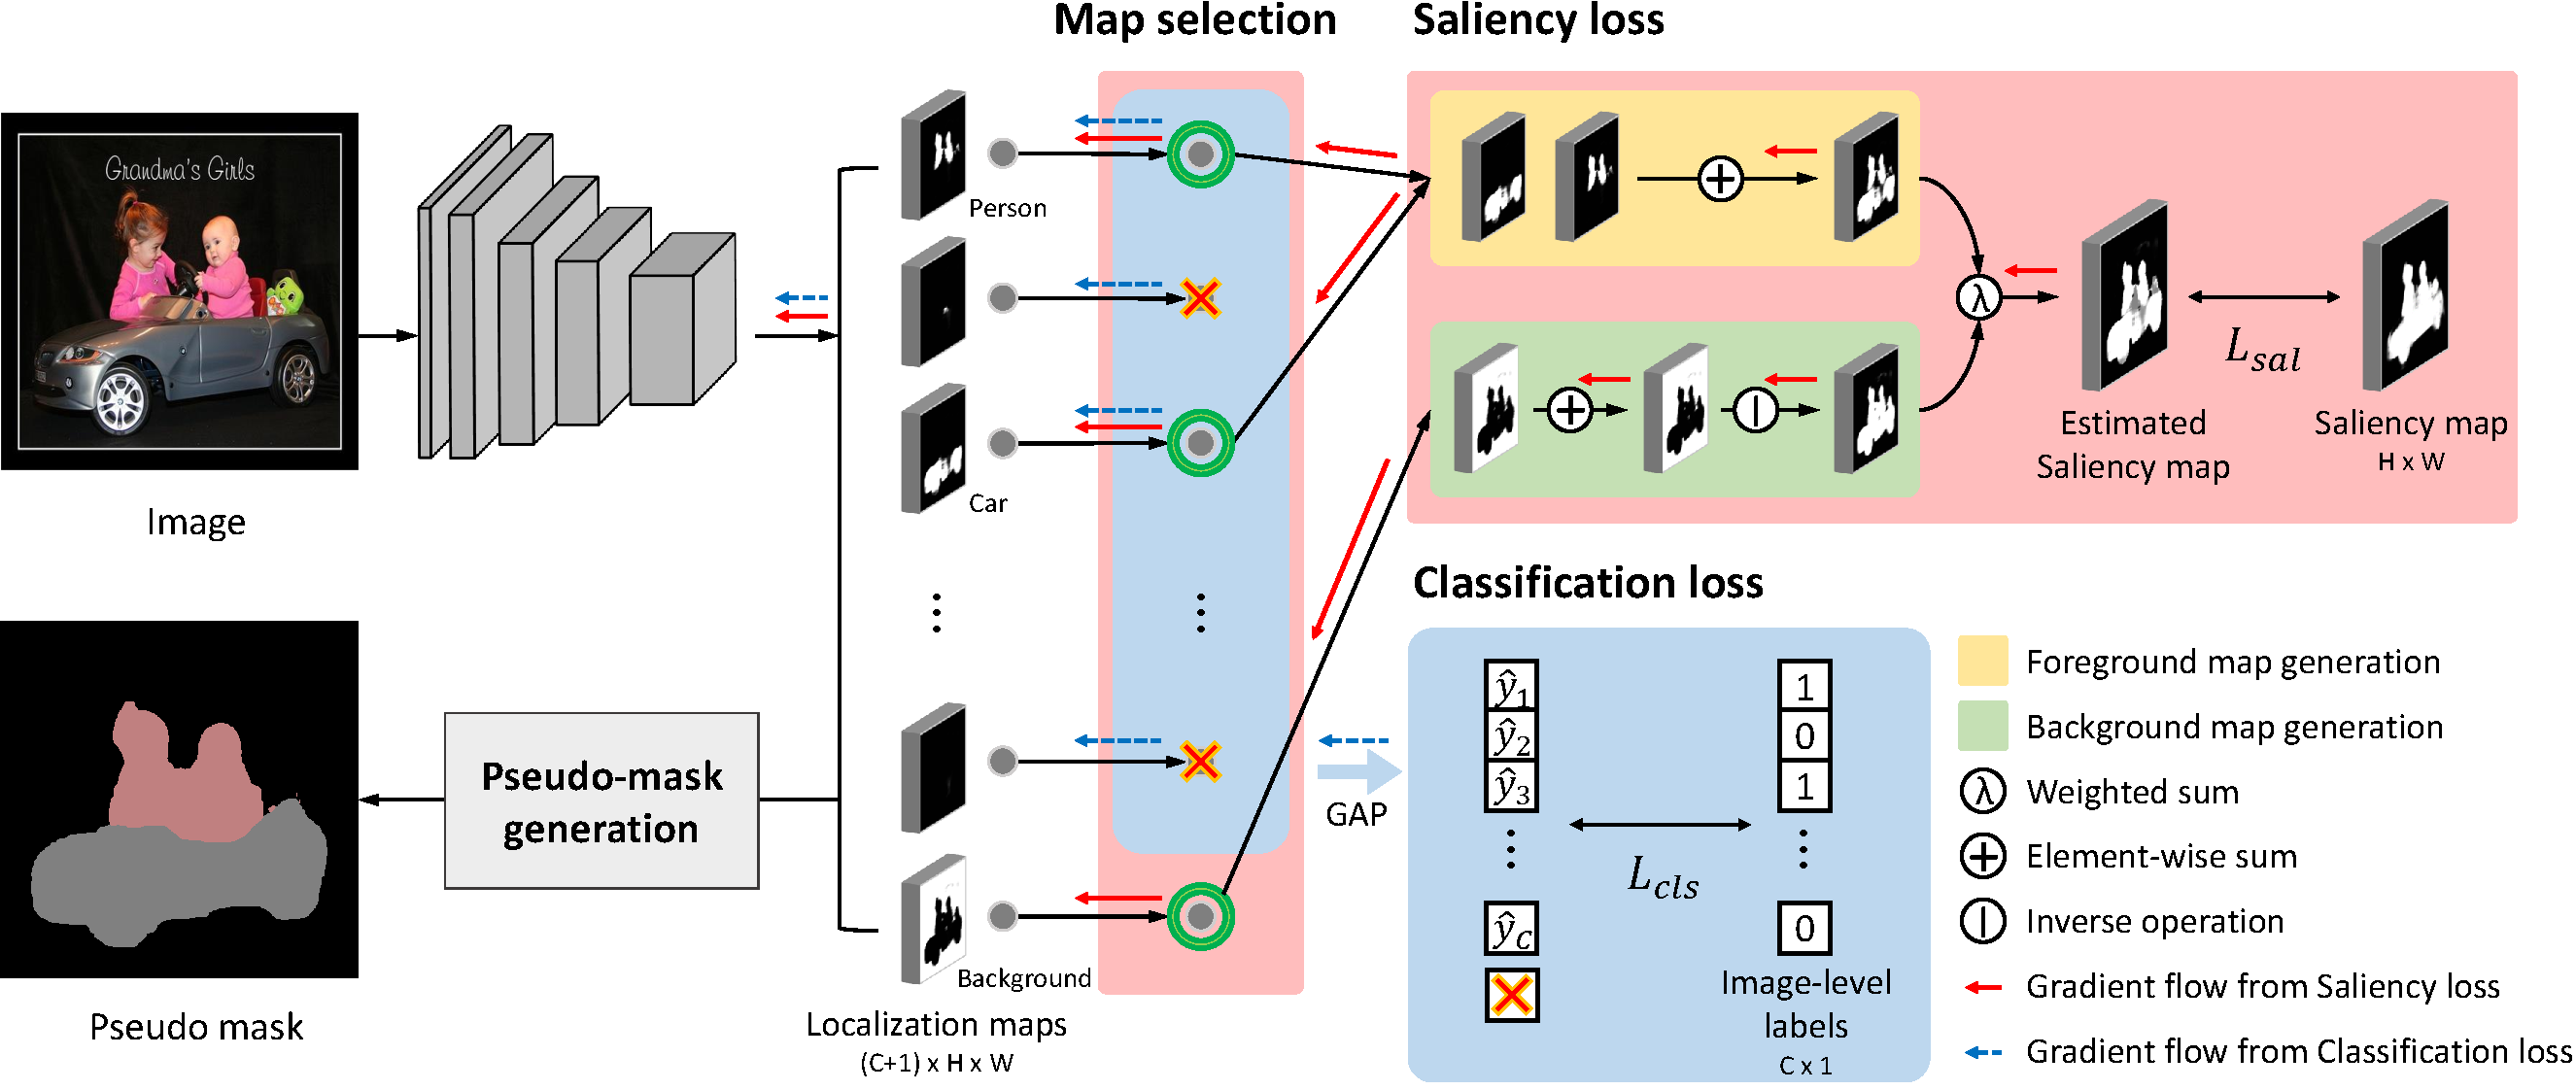
\includegraphics[width=16cm]{figures/framework.pdf}
\caption{我々のEPSの全体的なフレームワーク。$C+1$のローカライゼーションマップがバックボーンネットワークから生成されます。実際の顕著性マップは、既製の顕著性検出モデルから生成されます。ターゲットラベルのためのいくつかのローカライゼーションマップは、推定顕著性マップを生成するために選択的に使用されます(セクション~\ref{section3.2})。全体的なフレームワークは、顕著性損失と分類損失と共に共同で訓練されます(セクション~\ref{section3.3})。} \vspace{-2mm}
\label{fig:framework}
\end{figure*}


\vspace{1mm}
\noindent\textbf{基於顯著性的語義分割。}
顯著性檢測(SD)方法通過具有像素級註釋的外部顯著性數據集~\cite{hou2017deeply, xiao2018deep, zhao2019pyramid} 或圖像級註釋~\cite{wang2017learning} 生成區分圖像中前景和背景的顯著性圖。許多 WSSS 方法~\cite{fan2020cian, huang2018weakly, lee2019ficklenet, li2018tell, wei2017object, wei2018revisiting} 利用顯著性圖作為偽掩碼的背景線索。\cite{wei2016stc} 利用顯著性圖作為單物體圖像的完全監督。\cite{fan2018associating} 使用實例級顯著性圖來學習物體的相似性圖。\cite{chaudhry_dcsp_2017, wang2018weakly, yao2020saliency} 將顯著性圖與類別特定的注意力線索結合起來生成可靠的偽掩碼。\cite{zeng2019joint} 使用單一網絡聯合解決 WSSS 和 SD,以提高兩個任務的性能。我們的 EPS 可以歸類為基於顯著性的方法,但在以下原因中明顯區別於其他方法。大多數現有方法將顯著性圖作為偽掩碼的一部分或作為改進分類器中間特徵的隱式指導。相反,我們的方法利用顯著性圖作為定位圖的偽像素反饋。儘管 \cite{zeng2019joint} 在利用兩種互補信息的意義上與我們的工作最為相似,但他們既沒有解決共現問題,也沒有處理噪聲顯著性圖問題。

\section{提出的方法}

在本節中,我們提出了一個新的弱監督語義分割(WSSS)框架,稱為\emph{顯式偽像素監督(EPS)}。考慮到 WSSS 的兩個階段,第一階段是生成偽掩碼,第二階段是訓練分割模型。在這裡,我們的主要貢獻是生成準確的偽掩碼。遵循 WSSS 的慣例~\cite{fan2020learning,jiang2019integral,lee2019ficklenet,li2018tell,wang2020self,wei2017object},我們然後訓練一個分割模型,其中第一階段生成的偽掩碼用作監督。

\subsection{動機}
\label{section3.1}

EPS 的關鍵見解是充分利用兩種信息的互補性,即來自定位圖的物體身份和來自顯著性圖的邊界信息。為此,我們利用顯著性圖作為定位圖的偽像素反饋,針對目標標籤和背景。我們設計了一個具有額外背景類別的分類器,從而預測總共 $C+1$ 類別,如圖~\ref{fig:framework} 所示。使用該分類器,我們可以學習 $C+1$ 個定位圖,即 $C$ 個目標標籤的定位圖和一個背景定位圖。
我們接著解釋 EPS 如何解決 WSSS 中的邊界不匹配和共現問題。為了解決邊界不匹配問題,我們從 $C$ 定位圖估計前景圖,並將其與顯著性圖的前景匹配。這樣,目標標籤的定位圖可以從顯著性圖中接收偽像素反饋,從而改善物體的邊界。為了減少非目標物體的共現像素,我們還將背景的定位圖與顯著性圖匹配。由於背景的定位圖也從顯著性圖中接收偽像素反饋,共現像素可以成功地分配給背景;非目標物體的共現像素大多與背景重疊。這就是為什麼我們的方法可以將共現像素從目標物體中分離出來。
\begin{figure}[t]
\centering
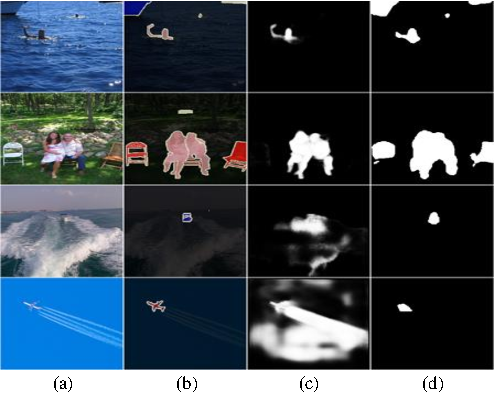
\includegraphics[width=8cm]{figures/fig_saliency_v2.pdf}
\caption{在 PASCAL VOC 2012 上估計的顯著性圖的質性範例。(a) 輸入圖像,(b) 真實值,(c) 來自 \cite{zhao2019pyramid} 的顯著性圖和 (d) 我們估計的顯著性圖。} \vspace{-2mm}
\label{fig:sal}
\end{figure}

最後,EPS 的目標函數由兩部分組成:通過顯著性圖的 {顯著性損失} $\mathcal{L}_{sal}$(在圖~\ref{fig:framework} 中以紅色框/箭頭標示)和通過圖像級標籤的 {多標籤分類損失} $\mathcal{L}_{cls}$(在圖~\ref{fig:framework} 中以藍色框/箭頭標示)。通過聯合訓練這兩個目標,我們可以將定位圖和顯著性圖的互補信息協同起來——我們觀察到通過我們的聯合訓練策略,彼此的噪聲和缺失信息得到了補充,如圖~\ref{fig:sal} 所示。例如,從現成模型~\cite{hou2017deeply,nguyen2019deepusps,zhao2019pyramid} 獲得的原始顯著性圖存在缺失和噪聲信息。另一方面,我們的結果成功恢復了缺失的物體(例如,船或椅子)並去除了噪聲(例如,水泡或飛機尾跡),這顯然比原始顯著性圖更好。因此,EPS 可以捕捉到更準確的物體邊界並將共現像素從目標物體中分離出來。這些優勢帶來了顯著的性能提升;表~\ref{tab:seg_quan_voc_resnet101} 報告稱,EPS 在分割準確性方面顯著超過現有模型,達到 3.8--10.6% 的增益。

\subsection{顯式偽像素監督}\label{section3.2}

我們解釋如何利用顯著性圖進行偽像素監督。顯著性圖的關鍵優勢在於提供物體輪廓,這可以更好地揭示物體邊界。為了利用這一特性,我們將顯著性圖與兩種情況匹配:前景和背景。為了使類別定位圖與顯著性圖可比,我們合併目標標籤的定位圖並生成前景圖,$\mathbf{M}_{fg} \in \mathbb{R}^{H \times W}$。我們也可以通過對背景圖進行反轉來表示前景,背景圖是背景標籤的定位圖 $\mathbf{M}_{bg} \in \mathbb{R}^{H \times W}$。(稍後,我們將解釋如何細化前景圖以解決噪聲顯著性圖問題。)

具體來說,我們使用 $\mathbf{M}_{fg}$ 和 $\mathbf{M}_{bg}$ 估計顯著性圖 $\mathbf{\hat{M}}_{s}$ 如下:\vspace{-1mm}
\begin{equation}
\label{eq_esimate_sal}
{\small
\begin{split}
\mathbf{\hat{M}}_{s} = \lambda\mathbf{M}_{fg} + (1-\lambda)(1-\mathbf{M}_{bg}),
\end{split}}\vspace{-1mm}
\end{equation}
\noindent 其中 $\lambda \in [0, 1]$ 是調整前景圖和背景圖反轉加權和的超參數。(在我們的實驗中,默認將 $\lambda$ 設置為 0.5,並在補充材料中提供了 $\lambda$ 的額外消融研究。)然後,我們將顯著性損失 $\mathcal{L}_{sal}$ 定義為我們估計的顯著性圖和實際顯著性圖之間的像素差異之和。($\mathcal{L}_{sal}$ 的正式定義在第~\ref{section3.3} 節中給出。)

值得注意的是,使用預訓練模型被視為弱監督學習,因此利用顯著性圖已被廣泛接受為 WSSS 中的常見做法。儘管如此,採用完全監督的顯著性檢測模型可能存在爭議,因為它們使用來自不同數據集的像素級註釋。在本文中,我們研究了不同顯著性檢測方法的效果;1)無監督和 2)完全監督的顯著性檢測模型(見第~\ref{section5.3} 節),並實證表明我們的方法使用其中任何一種都優於所有其他方法~\cite{fan2020learning,jiang2019integral,wang2018weakly, wei2016stc,yao2020saliency} 使用完全監督的顯著性模型。儘管現有方法在充分利用顯著性圖方面有限,我們的方法將顯著性圖作為偽像素監督,並將其作為邊界和共現像素的線索加以利用。

\vspace{1mm}
\noindent\textbf{處理顯著性偏差的地圖選擇。} 之前,我們假設前景地圖可以是目標標籤的定位地圖的聯集;背景地圖可以是背景標籤的定位地圖。然而,這樣的簡單選擇規則可能與現成模型計算的顯著性地圖不兼容。例如,來自\cite{zhao2019pyramid}的顯著性地圖經常忽略一些物體作為顯著物體(例如,圖~\ref{fig:concept}中火車旁的小人物)。這種系統性錯誤是不可避免的,因為顯著性模型學習了不同數據集的統計數據。除非考慮到這個錯誤,否則相同的錯誤可能會傳播到我們的模型中,導致性能下降。

為了解決系統性錯誤,我們開發了一種有效的策略,使用定位地圖和顯著性地圖之間的重疊率。具體來說,如果第 $i$ 個定位地圖 $\mathbf{M}_{i}$ 與顯著性地圖的重疊率超過 $\tau$\%,則將其分配給前景,否則分配給背景。形式上,前景和背景地圖計算如下:\vspace{-1mm}
\begin{equation}
\label{eq_map_selection}
{\small
\begin{split}
&\mathbf{M}_{fg} = \sum_{i=1}^{C} {y_{i} \cdot \mathbf{M}_{i} \cdot \mathbbm{1}[\mathcal{O}(\mathbf{M}_i, \mathbf{M}_{s}) > \tau]}, \\
&\mathbf{M}_{bg} = \sum_{i=1}^{C} {y_{i} \cdot \mathbf{M}_{i} \cdot \mathbbm{1}[\mathcal{O}(\mathbf{M}_i, \mathbf{M}_{s}) \le \tau]} + \mathbf{M}_{C+1},
\end{split}}\vspace{-1mm}
\end{equation}
\noindent 其中 $y \in \mathbb{R}^C$ 是二進制圖像級標籤,$\mathcal{O}(\mathbf{M}_i, \mathbf{M}_{s})$ 是計算 $\mathbf{M}_i$ 和 $\mathbf{M}_{s}$ 之間重疊率的函數。為此,我們首先將定位地圖和顯著性地圖二值化:對於像素 p,$\mathbf{B}_{k}(p) = 1$ 如果 $\mathbf{M}_{k}(p) > 0.5$;否則 $\mathbf{B}_{k}(p) = 0$。$\mathbf{B}_{i}$ 和 $\mathbf{B}_{s}$ 分別是對應於 $\mathbf{M}_i$ 和 $\mathbf{M}_{s}$ 的二值化地圖。然後,我們計算 $\mathbf{M}_i$ 和 $\mathbf{M}_{s}$ 之間的重疊率,即 $\mathcal{O}(\mathbf{M}_i ,\mathbf{M}_{s}) = |\mathbf{B}_i \cap \mathbf{B}_{s}| / |\mathbf{B}_{i}|$。我們設置 $\tau=0.4$,無論數據集和骨幹模型如何。在補充材料中,我們展示了我們的方法對 $\tau$ 的選擇具有魯棒性(即,$\tau$ 在 [0.3, 0.5] 之間顯示出可比的性能)。

我們將背景標籤的單一定位地圖與未選為前景的定位地圖結合起來。雖然這很簡單,但我們可以繞過顯著性地圖的錯誤,有效地訓練顯著性地圖忽略的一些物體。(在表~\ref{tab:strategy}中,我們報告了所提出策略克服顯著性地圖錯誤的有效性。)

\subsection{聯合訓練過程}\label{section3.3}

使用顯著性地圖和圖像級標籤,EPS 的整體訓練目標由兩部分組成,顯著性損失 $\mathcal{L}_{sal}$ 和分類損失 $\mathcal{L}_{cls}$。首先,顯著性損失 $\mathcal{L}_{sal}$ 通過測量實際顯著性地圖 $\mathbf{M}_{s}$ 和估計顯著性地圖 $\mathbf{\hat{M}}_{s}$ 之間的平均像素級距離來制定。\vspace{-1mm}
\begin{equation}
{\small
\label{loss_sal}
\mathcal{L}_{sal} = \frac{1}{H\cdot W}||\mathbf{M}_{s}-\mathbf{\hat{M}}_{s}||^{2},
}\vspace{-1mm}
\end{equation}
\noindent 其中 $\mathbf{M}_{s}$ 是從現成的顯著性檢測模型——在 DUTS 數據集~\cite{wang2017learning} 上訓練的 PFAN~\cite{zhao2019pyramid} 獲得的。請注意,我們的方法無論顯著性檢測模型如何,一貫優於所有先前的藝術。

接下來,分類損失是通過圖像級標籤 $y$ 和其預測 $\hat{y} \in \mathbb{R}^C$ 之間的多標籤軟邊緣損失計算的,這是每個目標類的定位地圖上的全局平均池化的結果。\vspace{-1mm}
\begin{equation}
{\small
\begin{split}
\label{loss_cls}
\mathcal{L}_{cls}= - \frac{1}{C} \sum_{i=1}^{C} y_i \log{\sigma(\hat{y_i})} + (1-y_i) \log{(1 - \sigma(\hat{y_i}))},
\end{split}}\vspace{-1mm}
\end{equation}
\noindent 其中 $\sigma(\cdot)$ 是 sigmoid 函數。最後,總訓練損失是多標籤分類損失和顯著性損失的總和,即 $\mathcal{L}_{total} = \mathcal{L}_{cls} + \mathcal{L}_{sal}$。
如圖~\ref{fig:framework}所示,$\mathcal{L}_{sal}$ 涉及更新 $C+1$ 類別的參數,包括目標物體和背景。同時,$\mathcal{L}_{cls}$ 僅評估 $C$ 類別的標籤預測,不包括背景類別——來自 $\mathcal{L}_{cls}$ 的梯度不會流入背景類別。然而,背景類別的預測可以被 $\mathcal{L}_{cls}$ 隱式影響,因為它監督分類器的訓練。

\section{實驗設置}
\noindent
\textbf{數據集}。我們在兩個流行的基準數據集上進行實證研究,分別是 PASCAL VOC 2012~\cite{everingham2015pascal} 和 MS COCO 2014~\cite{lin2014microsoft}。PASCAL VOC 2012 包含 21 個類別(即 20 個物體和背景),訓練集、驗證集和測試集分別有 1,464、1,449 和 1,456 張圖像。按照語義分割的常見做法,我們使用擴充的訓練集,其中包含 10,582 張圖像~\cite{hariharan2011semantic}。接下來,COCO 2014 包含 81 個類別,包括一個背景,訓練和驗證集分別有 82,081 和 40,137 張圖像,其中不包含目標類別的圖像已被排除,如~\cite{choe2020attention} 所述。由於某些物體的真實分割標籤相互重疊,我們採用 COCO-Stuff~\cite{caesar2018coco} 的真實分割標籤,該標籤解決了同一 COCO 數據集上的重疊問題。

\vspace{0.5mm}
\noindent
\textbf{評估協議}。我們在 PASCAL VOC 2012 的驗證集和測試集以及 COCO 2014 的驗證集上驗證我們的方法。PASCAL VOC 2012 測試集的評估結果來自官方 PASCAL VOC 評估服務器。此外,我們採用平均交集-聯合(mIoU)來衡量分割模型的準確性。

\vspace{0.5mm}
\noindent
\textbf{實現細節}。我們選擇 ResNet38~\cite{wu2019wider} 作為我們方法的骨幹網絡,輸出步幅為 8。所有骨幹模型均在 ImageNet~\cite{deng2009imagenet} 上進行預訓練。我們使用批量大小為 8 的 SGD 優化器。我們的方法訓練到 20k 次迭代,學習率為 0.01(最後一個卷積層為 0.1)。對於數據增強,我們使用隨機縮放、隨機翻轉和隨機裁剪到 $448 \times 448$。對於分割網絡,我們採用 DeepLab-LargeFOV (V1)~\cite{chen2014semantic} 和 DeepLab-ASPP (V2)~\cite{chen2017deeplab},以及 VGG16 和 ResNet101 作為其骨幹網絡。具體來說,我們使用四個分割網絡:基於 VGG16 的 DeepLab-V1 和 DeepLab-V2,基於 ResNet101 的 DeepLab-V1 和 DeepLab-V2。更詳細的設置在補充材料中。

\section{實驗結果}

\subsection{處理邊界和共現問題}\label{section:5.1}

\noindent\textbf{邊界不匹配問題}。為了驗證偽掩碼的邊界,我們將邊界的質量與最先進的方法~\cite{chen2020boundary, wang2020self, zhou2016learning} 進行比較。我們利用 SBD~\cite{hariharan2011semantic},該數據集提供了邊界註釋和 PASCAL VOC 2011 的邊界基準。如~\cite{chen2020boundary} 所述,邊界的質量以類別無關的方式進行評估,通過計算偽掩碼的邊緣來自拉普拉斯邊緣檢測器。然後,通過測量召回率、精確率和 F1 分數來評估邊界質量,將預測的邊界與真實邊界進行比較。表~\ref{tab:boundary} 報告了我們的方法在所有三個指標上大大超過其他方法。圖~\ref{fig:ablation} 中的定性示例顯示,我們的方法可以比所有其他方法捕捉到更準確的邊界。

\begin{figure}[t]
\centering
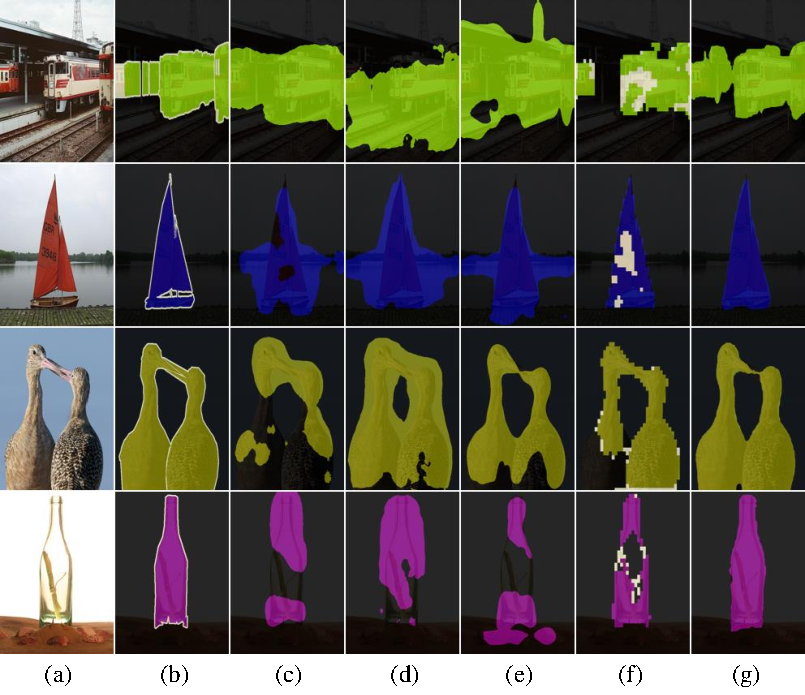
\includegraphics[width=8cm]{figures/fig_ablation.pdf}
\caption{Qualitative comparison for pseudo-masks on PASCAL VOC 2012. (a) Input images, (b) groundtruth, (c) CAM, (d) SEAM, (e) ICD, (f) SGAN and (g) our EPS.}
\label{fig:ablation} \vspace{-3mm}
\end{figure}


\begin{table}[]
\centering
{\small
\begin{tabular}{@{}lccc@{}}
\toprule
\multicolumn{1}{c}{方法}                      & 召回率(\%) & 精确率(\%) & F1-分数(\%) \\ \midrule
\multicolumn{1}{l}{CAM~\cite{zhou2016learning}\textsubscript{CVPR'16}} & 22.3        & 35.8           & 27.5           \\
\multicolumn{1}{l}{SEAM~\cite{wang2020self}\textsubscript{CVPR'20}}    & 40.2        & 45.0           & 42.5           \\
\multicolumn{1}{l}{BES~\cite{chen2020boundary}\textsubscript{ECCV'20}} & 45.5        & 46.4           & 45.9           \\
\multicolumn{1}{l}{我们的 EPS}                        & 60.0        & 73.1          & 65.9           \\ \bottomrule
\end{tabular}
}
\vspace{2mm}
\caption{在 SBD trainval 集上评估的边界准确性。请注意,BES 的结果是从~\cite{chen2020boundary}中提出的边界预测网络测量的。} \vspace{-2mm}
\label{tab:boundary}
\end{table}


\vspace{1mm}
\noindent \textbf{共現問題}。如幾項研究中所討論的~\cite{huang2018weakly, kolesnikov2016seed, li2018tell, oh2017exploiting},我們觀察到在 PASCAL VOC 2012 中,一些背景類別經常與目標物體一起出現。我們通過使用 PASCAL-CONTEXT 數據集~\cite{mottaghi2014role} 進行定量分析,該數據集提供了整個場景的像素級註釋(例如,~\emph{水} 和 ~\emph{鐵路})。我們選擇了三對共現對;\emph{船} 與 \emph{水},\emph{火車} 與 \emph{鐵路},以及 \emph{火車} 與 \emph{平台}。我們比較目標類別的 IoU 和目標類別與其共現類別之間的 \emph{混淆比率}。混淆比率衡量共現類別被錯誤預測為目標類別的程度。混淆比率 $m_{k,c}$ 通過 $m_{k,c} = FP_{k,c}/TP_{c}$ 計算,其中 ${FP_{k,c}}$ 是共現類別 $k$ 被錯誤分類為目標類別 $c$ 的像素數,$TP_{c}$ 是目標類別 $c$ 的真陽性像素數。關於共現問題的更詳細分析在補充材料中。
Table~\ref{tab:co_quantitative_v4} 報告指出,EPS 一直顯示出比其他方法更低的混淆比率。SGAN~\cite{yao2020saliency} 的混淆比率與我們的方法相當相似,但我們的方法在 IoU 方面更準確地捕捉到目標類別。有趣的是,SEAM 顯示出高混淆比率,甚至比 CAM 更糟糕。這是因為 SEAM~\cite{wang2020self} 通過應用自我監督訓練來學習覆蓋目標物體的全部範圍,這很容易被目標物體的重合像素所誤導。與此同時,CAM 只捕捉到目標物體的最具辨識性的區域,並不覆蓋較不具辨識性的部分,例如重合類別。我們也可以在圖~\ref{fig:ablation} 中觀察到這一現象。

% 請將以下所需的套件添加到您的文件前言:
% \usepackage{booktabs}

\newcommand{\R}{\textcolor{red}}
\newcommand{\B}{\textcolor{blue}}

\begin{table}[]
\centering
{\small
\begin{tabular}{@{}llll@{}}
\toprule
\multicolumn{1}{c}{\multirow{2}{*}{方法}} & \multicolumn{1}{c}{~\emph{船} w/}   & \multicolumn{1}{c}{~\emph{火車} w/}  & \multicolumn{1}{c}{~\emph{火車} w/}  \\
& \multicolumn{1}{c}{~\emph{水}} & \multicolumn{1}{c}{~\emph{鐵路}}          & \multicolumn{1}{c}{~\emph{平台}}  \\ \midrule
\multicolumn{1}{l}{CAM~\cite{zhou2016learning}\textsubscript{CVPR'16}}              & \B{0.74} (33.1)   & \B{0.11} (52.9)   & \multicolumn{1}{l}{\B{0.09} (49.6)}   \\
\multicolumn{1}{l}{SEAM~\cite{wang2020self}\textsubscript{CVPR'20}}                 & \B{1.13} (30.7)   & \B{0.24} (48.6)   & \multicolumn{1}{l}{\B{0.20} (45.5)}   \\
\multicolumn{1}{l}{ICD~\cite{fan2020learning}\textsubscript{CVPR'20}}               & \B{0.47} (41.4)   & \B{0.11} (56.7)   & \multicolumn{1}{l}{\B{0.09} (49.2)}   \\
\multicolumn{1}{l}{SGAN~\cite{yao2020saliency}\textsubscript{ACCESS'20}}            & \B{0.10} (42.3)   & \B{0.02} (48.8)   & \multicolumn{1}{l}{\B{0.01} (36.3)}   \\
\multicolumn{1}{l}{我們的 EPS}                                                         & \B{0.10} (55.0)   & \B{0.02} (78.1)   & \multicolumn{1}{l}{\B{0.01} (73.0)}   \\ \bottomrule
\end{tabular}
}
\vspace{2mm}
\caption{與現有代表性方法處理共現問題的比較。每個條目是 {$m_{k,c}$} 在~\B{藍色}中(越低越好),括號中的 IoU(越高越好)。} \vspace{-2mm}
\label{tab:co_quantitative_v4}

\end{table}

\begin{table}[]
%\resizebox{\columnwidth}{!}{%
\centering

{\small
\begin{tabular}{@{}ccccc@{}}
\toprule
                            & 基线  & 简单   & 预定义   & 我们的自适应 \\ \midrule
\multicolumn{1}{l}{mIoU}    &66.1       & 66.5      & 67.9          & 69.4   \\ \bottomrule
\end{tabular}
}
\vspace{2mm}
\caption{地图选择策略的效果。使用不同地图选择策略的伪掩码的准确性在 PASCAL VOC 2012 训练集上进行评估。} \vspace{-2mm}
\label{tab:strategy}
\end{table}


\subsection{地圖選擇策略的效果}
我們評估了我們的地圖選擇策略在減少顯著性地圖錯誤方面的有效性。我們將三種不同的地圖選擇策略與不使用地圖選擇模塊的基線進行比較。作為簡單策略,前景地圖是所有物體定位地圖的聯集;背景地圖等於背景類別的定位地圖(即簡單策略)。接下來,我們遵循簡單策略,但有以下例外。幾個預定類別(例如,\emph{沙發}、\emph{椅子}和\emph{餐桌})的定位地圖被分配到背景地圖(即預定類別策略)。最後,所提出的選擇方法利用定位地圖和顯著性地圖之間的重疊比率,如第~\ref{section3.2} 節所述(即我們的自適應策略)。

\begin{figure*}[t]
\centering
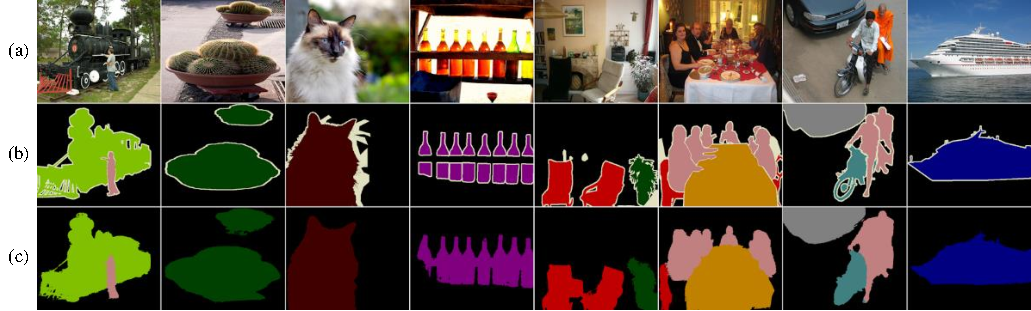
\includegraphics[width=17cm]{figures/segmentation_voc.pdf}
\caption{PASCAL VOC 2012 上分割结果的定性示例。(a) 输入图像,(b) 真实值和 (c) 我们的 EPS。}\vspace{-2mm}
\label{fig:seg_qual_voc}
\end{figure*}

\begin{table}[]
\centering
{\small
\begin{tabular}{@{}lccc@{}}
\toprule
\multicolumn{1}{c}{\multirow{2}{*}{Method}}         & w/o           & w/ &                                  w/ \\
                                                    & refinement    & CRF~\cite{krahenbuhl2011efficient}    & AffinityNet~\cite{ahn2018learning}    \\ \midrule
\multicolumn{1}{l}{CAM~\cite{zhou2016learning}\textsubscript{CVPR'16}}     & 48.0          & -                                     & 58.1                                  \\
\multicolumn{1}{l}{SEAM~\cite{wang2020self}\textsubscript{CVPR'20}}        & 55.4          & 56.8                                  & 63.6                                  \\
\multicolumn{1}{l}{ICD~\cite{chen2020boundary}\textsubscript{CVPR'20}*}     & 59.9          & 62.2                                  & -                                     \\
\multicolumn{1}{l}{SGAN~\cite{yao2020saliency}\textsubscript{ACCESS'20}*}     & 62.8          & -                                     & -                                     \\
\multicolumn{1}{l}{Our EPS}                            & 69.4          & 71.4                                  & 71.6                                  \\ \bottomrule
\end{tabular}
}
\vspace{2mm}
\caption{PASCAL VOC 2012のトレインセットで評価された擬似マスクの精度(mIoU)。*は低信頼度のピクセルが無視されることを示します。他の方法はすべてのピクセルを評価に使用します。} \vspace{-3mm}
\label{tab:refinement}
\end{table}


Table~\ref{tab:strategy} 顯示,我們的自適應策略可以有效地處理顯著性地圖的系統偏差。簡單策略意味著在從定位地圖生成估計的顯著性地圖時沒有考慮偏差。在這種情況下,偽掩碼的性能下降,特別是在\emph{沙發}、\emph{椅子}或\emph{餐桌}類別上。使用預定類別的性能顯示,通過忽略顯著性地圖中缺失的類別可以減少偏差。然而,由於需要人類觀察者的手動選擇,這不太實用,並且無法對每張圖像做出最佳決策。與此同時,我們的自適應策略可以自動處理偏差,並為給定的顯著性地圖做出更有效的決策。

\subsection{與最先進技術的比較}
\label{section5.3}

\noindent \textbf{偽掩碼的準確性。} 我們通過聚合來自不同尺度圖像的預測結果來採用多尺度推理,這是~\cite{ahn2018learning,wang2020self} 中常用的做法。然後,我們通過將我們的 EPS 與基線 CAM~\cite{zhou2016learning} 和三種最先進的方法,即 SEAM~\cite{wang2020self}、ICD~\cite{fan2020learning} 和 SGAN~\cite{yao2020saliency} 進行比較,來評估訓練集中的偽掩碼的準確性。在 WSSS 中,測量訓練集中的偽掩碼的準確性是一種常見的協議,因為訓練集的偽掩碼用於監督分割模型。Table~\ref{tab:refinement} 總結了偽掩碼的準確性,並表明我們的方法明顯優於所有現有方法,差距達到 7--21%。圖~\ref{fig:ablation} 可視化了偽掩碼的質量示例,證實我們的方法顯著改善了物體邊界,並在偽掩碼的質量方面顯著優於三種最先進的方法。我們的方法可以捕捉到物體的精確邊界(第二行),因此自然地覆蓋物體的全部範圍(第三行),並且還減少了重合像素(第一行)。更多我們方法的示例和失敗案例在補充材料中提供。

\begin{table}[]
\normalsize
\centering
{\small
\begin{tabular}{@{}lccll@{}}
\toprule
\multicolumn{1}{c}{방법}                                                              & 세그.      & 지원.  & \multicolumn{1}{c}{val} & \multicolumn{1}{c}{test} \\ \midrule
\multicolumn{1}{l}{SEC~\cite{kolesnikov2016seed}\textsubscript{ECCV'16}}                & V1        & I.    & 50.7                    & 51.7                     \\
\multicolumn{1}{l}{AffinityNet~\cite{ahn2018learning}\textsubscript{CVPR'18}}           & V1        & I.    & 58.4                    & 60.5                     \\
\multicolumn{1}{l}{ICD~\cite{fan2020learning}\textsubscript{CVPR'20}}                   & V1        & I.    & 61.2                    & 60.9                     \\
\multicolumn{1}{l}{BES~\cite{chen2020boundary}\textsubscript{ECCV'20}}                  & V1        & I.    & 60.1                    & 61.1                     \\
\multicolumn{1}{l}{GAIN~\cite{li2018tell}\textsubscript{CVPR'18}}                       & V1        & I.+S. & 55.3                    & 56.8                     \\
\multicolumn{1}{l}{MCOF~\cite{wang2018weakly}\textsubscript{CVPR'18}}                   & V1        & I.+S. & 56.2                    & 57.6                     \\
\multicolumn{1}{l}{SSNet~\cite{zeng2019joint}\textsubscript{ICCV'19}}                   & V1        & I.+S. & 57.1                    & 58.6                     \\
\multicolumn{1}{l}{DSRG~\cite{huang2018weakly}\textsubscript{CVPR'18}}                  & V2        & I.+S. & 59.0                    & 60.4                     \\
\multicolumn{1}{l}{SeeNet~\cite{hou2018self}\textsubscript{NeurIPS'18}}                 & V1        & I.+S. & 61.1                    & 60.7                     \\
\multicolumn{1}{l}{MDC~\cite{wei2018revisiting}\textsubscript{CVPR'18}}                 & V1        & I.+S. & 60.4                    & 60.8                     \\
\multicolumn{1}{l}{FickleNet~\cite{lee2019ficklenet}\textsubscript{CVPR'18}}            & V2        & I.+S. & 61.2                    & 61.9                     \\
\multicolumn{1}{l}{OAA~\cite{jiang2019integral}\textsubscript{ICCV'19}}                 & V1        & I.+S. & 63.1                    & 62.8                     \\
\multicolumn{1}{l}{ICD~\cite{fan2020learning}\textsubscript{CVPR'20}}                   & V1        & I.+S. & 64.0                    & 63.9                     \\
\multicolumn{1}{l}{Multi-Est.~\cite{fan2020employing}\textsubscript{ECCV'20}}           & V1        & I.+S. & 64.6                    & 64.2                     \\
\multicolumn{1}{l}{Split. \& Merge.~\cite{zhang2020splitting}\textsubscript{ECCV'20}}   & V2        & I.+S. & 63.7                    & 64.5                     \\
\multicolumn{1}{l}{SGAN~\cite{yao2020saliency}\textsubscript{ACCESS'20}}                & V2        & I.+S. & 64.2                    & 65.0                     \\ \midrule
\multicolumn{1}{l}{\multirow{2}{*}{우리의 EPS}}                                            & V1        & I.+S. & 66.6                    & \textbf{67.9}            \\
\multicolumn{1}{l}{}                                                                    & V2        & I.+S. & \textbf{67.0}           & 67.3                     \\ \bottomrule

\end{tabular}
}
\vspace{2mm}
\caption{PASCAL VOC 2012에서의 세그멘테이션 결과 (mIoU). 모든 결과는 VGG16을 기반으로 합니다. 모든 실험에서 최고의 점수는 굵게 표시되어 있습니다.}\vspace{-3mm}
\label{tab:seg_quan_voc_vgg16}
\end{table}

\begin{table}[]
\normalsize
\centering
{\small
\begin{tabular}{@{}lccll@{}}
\toprule
\multicolumn{1}{c}{Method}                                                              & Seg.      & Sup.  & \multicolumn{1}{c}{val} & \multicolumn{1}{c}{test} \\ \midrule
\multicolumn{1}{l}{ICD~\cite{fan2020learning}\textsubscript{CVPR'20}}                   & V1        & I.    & 64.1                    & 64.3                     \\ 
\multicolumn{1}{l}{SC-CAM~\cite{chang2020weakly}\textsubscript{CVPR'20}}                & V1        & I.    & 66.1                    & 65.9                     \\
\multicolumn{1}{l}{BES~\cite{chen2020boundary}\textsubscript{ECCV'20}}                  & V2        & I.    & 65.7                    & 66.6                     \\
\multicolumn{1}{l}{LIID~\cite{liu2020leveraging}\textsubscript{TPAMI'20}}                  & V2        & I.    & 66.5                    & 67.5                     \\
\multicolumn{1}{l}{MCOF~\cite{wang2018weakly}\textsubscript{CVPR'18}}                   & V1        & I.+S. & 60.3                    & 61.2                     \\
\multicolumn{1}{l}{SeeNet~\cite{hou2018self}\textsubscript{NeurIPS'18}}                 & V1        & I.+S. & 63.1                    & 62.8                     \\
\multicolumn{1}{l}{DSRG~\cite{huang2018weakly}\textsubscript{CVPR'18}}                  & V2        & I.+S. & 61.4                    & 63.2                     \\
\multicolumn{1}{l}{FickleNet~\cite{lee2019ficklenet}\textsubscript{CVPR'18}}            & V2        & I.+S. & 64.9                    & 65.3                     \\
\multicolumn{1}{l}{OAA~\cite{jiang2019integral}\textsubscript{ICCV'19}}                 & V1        & I.+S. & 65.2                    & 66.4                     \\
\multicolumn{1}{l}{Multi-Est.~\cite{fan2020employing}\textsubscript{ECCV'19}}           & V1        & I.+S. & 67.2                    & 66.7                     \\
\multicolumn{1}{l}{MCIS~\cite{sun2020mining}\textsubscript{ECCV'20}}                    & V1        & I.+S. & 66.2                    & 66.9                     \\
\multicolumn{1}{l}{SGAN~\cite{yao2020saliency}\textsubscript{ACCESS'20}}                & V2        & I.+S. & 67.1                    & 67.2                     \\
\multicolumn{1}{l}{ICD~\cite{fan2020learning}\textsubscript{CVPR'20}}                   & V1        & I.+S. & 67.8                    & 68.0                     \\ \midrule
\multicolumn{1}{l}{\multirow{2}{*}{Our EPS}}                                            & V1        & I.+S. & \textbf{71.0}           & \textbf{71.8}            \\
\multicolumn{1}{l}{}                                                                    & V2        & I.+S. & 70.9                    & 70.8                     \\ \bottomrule
\end{tabular}
}
\vspace{2mm}
\caption{PASCAL VOC 2012에서의 세그멘테이션 결과 (mIoU). 모든 결과는 ResNet101을 기반으로 합니다.}\vspace{-2mm}
\label{tab:seg_quan_voc_resnet101}
\end{table}

\begin{figure*}[t]
\centering
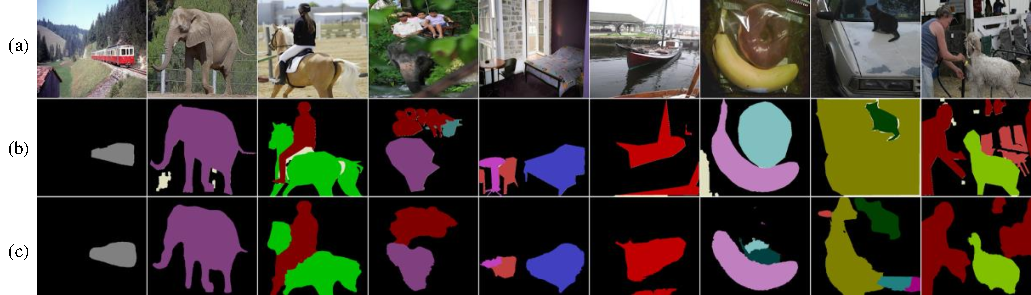
\includegraphics[width=17cm]{figures/segmentation_coco.pdf}
\caption{MS COCO 2014에서의 세분화 결과에 대한 정성적 예시입니다. (a) 입력 이미지, (b) 정답 및 (c) 우리의 EPS.}\vspace{-2mm}
\label{fig:seg_qual_coco} 
\end{figure*}


\vspace{1mm}
\noindent \textbf{分割地圖的準確性}。先前的方法~\cite{ahn2018learning, fan2020learning, wang2020self} 生成偽掩碼並使用 CRF 後處理算法~\cite{krahenbuhl2011efficient} 或親和網絡~\cite{ahn2018learning} 進行細化。與此同時,如 Table~\ref{tab:refinement} 所示,我們生成的偽掩碼足夠準確,因此我們在不進行任何額外的偽掩碼細化的情況下訓練分割網絡。我們在 Pascal VOC 2012 數據集上的四個分割網絡上廣泛評估並精確比較我們的方法與其他方法。

% Please add the following required packages to your document preamble:
% \usepackage{booktabs}
\begin{table}[]
\centering
{\small
\begin{tabular}{@{}lccc@{}}
\toprule
\multicolumn{1}{c}{Method}                                                  &Seg.       &Sup.   & \multicolumn{1}{c}{val}           \\ \midrule
\multicolumn{1}{l}{SEC~\cite{kolesnikov2016seed}\textsubscript{ECCV'16}}    & V1        &I.     & \multicolumn{1}{c}{22.4}          \\
\multicolumn{1}{l}{DSRG~\cite{huang2018weakly}\textsubscript{CVPR'18}}      & V2        &I.+S.  & \multicolumn{1}{c}{26.0}          \\
\multicolumn{1}{l}{ADL~\cite{choe2020attention}\textsubscript{TPAMI'20}}    & V1        &I.+S.  & \multicolumn{1}{c}{30.8}          \\
\multicolumn{1}{l}{SGAN~\cite{yao2020saliency}\textsubscript{ACESS'20}}     & V2        &I.+S.  & \multicolumn{1}{c}{33.6}          \\ \midrule
\multicolumn{1}{l}{Our EPS}                                                 & V2        &I.+S.  & \multicolumn{1}{c}{\textbf{35.7}} \\ \bottomrule
\end{tabular}
}
\vspace{2mm}
\caption{Segmentation results (mIoU) on MS COCO 2014. All results are based on VGG16.}\vspace{-2mm}
\label{tab:seg_quantitative_coco}
\end{table}
我們的方法在分割網絡方面表現顯著優於其他方法。表~\ref{tab:seg_quan_voc_vgg16} 報告顯示,我們的方法在相同的 VGG16 骨幹下比其他方法更準確。此外,我們在 VGG16 上的結果與基於更強大骨幹的其他現有方法(\ie 表~\ref{tab:seg_quan_voc_resnet101} 中的 ResNet101)相當甚至更優。我們的方法也顯示出對現有方法的明顯改進。最後,表~\ref{tab:seg_quan_voc_resnet101} 顯示,我們的方法(在基於 ResNet101 的 DeepLab-V1 與顯著性圖下)在 PASCAL VOC 2012 數據集上達到了新的最先進性能(驗證集為 71.0,測試集為 71.8)。我們強調,現有最先進模型所取得的增益約為 1\%。同時,我們的方法比之前的最佳記錄高出超過 3\% 的增益。圖~\ref{fig:seg_qual_voc} 可視化了我們在 PASCAL VOC 2012 上的分割結果的質量示例。這些結果證實了我們的方法提供了準確的邊界並成功解決了共現問題。

在表~\ref{tab:seg_quantitative_coco} 中,我們進一步在 COCO 2014 數據集中評估了我們的方法。我們使用基於 VGG16 的 DeepLab-V2 作為分割網絡來與 SGAN~\cite{yao2020saliency} 進行比較,該模型是 COCO 數據集中的最先進 WSSS 模型。我們的方法在驗證集上達到了 35.7 mIoU,比 SGAN~\cite{yao2020saliency} 高出 1.9\%。因此,我們在 COCO 2014 數據集中達到了新的最先進準確性。這些在兩個數據集上超越現有最先進技術的出色表現證實了我們方法的有效性;通過充分利用定位圖和顯著性圖,它成功地正確捕捉了目標對象的整體,並彌補了現有模型的不足。圖~\ref{fig:seg_qual_coco} 顯示了 COCO 2014 數據集上的分割結果的質量示例。我們的方法在少數對象出現而無遮擋時表現良好,但在處理許多小對象時效果較差。更多示例和失敗案例在補充材料中提供。

\vspace{1mm}
\noindent \textbf{顯著性檢測模型的效果}。為了研究不同顯著性檢測模型的效果,我們採用了三種顯著性模型;PFAN~\cite{zhao2019pyramid}(我們的默認),DSS~\cite{hou2017deeply} 用於 OAA~\cite{jiang2019integral} 和 ICD~\cite{fan2020learning},以及 USPS~\cite{nguyen2019deepusps}(\ie,無監督檢測模型)。在基於 Resnet101 的 DeepLab-V1 下的分割結果(mIoU)分別為 71.0/71.8(PFAN),70.0/70.1(DSS),和 68.8/69.9(USPS)(驗證集和測試集)。這些分數支持我們的 EPS 使用任何三種不同的顯著性模型仍然比表~\ref{tab:seg_quan_voc_resnet101} 中的所有其他方法更準確。值得注意的是,我們的 EPS 使用無監督顯著性模型優於所有使用監督顯著性模型的現有方法。

\section{結論}
我們提出了一種新穎的弱監督分割框架,即 \emph{顯式偽像素監督(EPS)}。受定位圖和顯著性圖之間互補關係的啟發,我們的 EPS 從結合顯著性圖和定位圖的偽像素反饋中學習。由於我們的聯合訓練方案,我們成功地補充了雙方的噪音或缺失信息。因此,我們的 EPS 能夠捕捉精確的對象邊界並丟棄非目標對象的共現像素,顯著提高了偽掩碼的質量。廣泛的評估和各種案例研究證明了我們的 EPS 的有效性和出色的性能,為 PASCAL VOC 2012 和 MS COCO 2014 數據集上的 WSSS 提供了新的最先進準確性。

\noindent\textbf{致謝。}
我們感謝 Duhyeon Bang 和 Junsuk Choe 的反饋。這項研究得到了韓國 MSIP 資助的 NRF 基礎科學研究計劃(NRF-2019R1A2C2006123,2020R1A4A1016619),由 MSIT 資助的 IITP 資助(2020-0-01361,人工智能研究生院計劃(延世大學)),以及由韓國政府資助的韓國醫療設備開發基金資助(項目編號:202011D06)。

{\small
\bibliographystyle{ieee_fullname}
\bibliography{egbib}
}

\end{document}
